\chapter{Techniques}
\label{Chapter4}
\lhead{Chapter 4. \emph{Codes}}

Throughout this thesis my goals were to identify SLSNe in a number of surveys. I have approached this problem using a variaty of tools and techniques which I describe in this chapter. The methods of classification SLSN described in this chapter span a number of methods. In the early parts of this thesis I used an approached based on modelling of SLSNe using the popular spin-down of a magnetar model \sref{sec:SLAP}. While this technique was successful in identifying a new SLSN in the SNLS it was found to be insufficient in the case of mode diverse but also noisy DES data. To solve this problem I have followed a popular path for classification style problems by approaching it using a machine learning approach. It is the preparation for the sample building methods, described further in \cref{Chapter5}, that form the second part of this chapter. The use of machine learning means that the majority of the work is not put into the understanding of the parameter space of the model applied to the data and any potential cuts that need to be made by currating and cleaning the data. Our approach is to simulate DES using all tranient models that are currently availabe to us. This includes similating SNIa, CCSN, SLSN as well as random noise and AGN activity.

While the models of SNIa are mature and ready to be applied to our work the simulations of CCSN could not have been accieved that easily. CCSN are usually faster and fainter than SNIa resulting is a significantly smaller sample of well observed objects. Most of them are also not observed using the same spectoscopic thoroughness making the a less understood class of objects. In recent years the interest in modeling this objects has increased dramatically with projects such as LSST underway. In this chapter I describe our approach to producing templates of CCSN as well as simulating them in a number of surveys. This project has originally been started as part of the LSST transients classification challenge however later I have applied it to DES to produce samples of both hydrogen rich and poor CCSN.

The last, but perhaps the most key, technique descrined in this chapter is Gaussian Processing. As the DES data was not observed on regular cadance, it would be impossible to apply any machine learning technique to good success to the row data. We used GPs as a method of modelling the confidence regions of the underlying light curves for the observed and simulated DES objects in a model-independant way. This was key as at the next stage of the process it would be "BAD" if instead of classifing the objects we uncover the underlying model instead of the data itself.

This chapter is divided in the following way. I begin by describing the method of modelling of SLSNe using the magnetar model in conjunction with SED templates. I then follow this by a discussion of the method as applied to the search for SLSNe in DES as well as their pre-peak 'bumps' and other rapidly evolving transients. Next, I describe the process of Gaussian Processing light curves as a model-independant approach to approximating the original data. Finally I describe the technique behind simulating samples of CCSN as used for machine learning classification of SLSNe.

\section{Modeling SLSN Light Curves} \label{sec:SLAP}
Throughout this thesis the modelling of SLSNe light curves plays a pivotal role. The measurement of the rate of SLSNe presented in \cref{Chapter3} as well as the search for SLSNe in DES described in \cref{Chapter5,Chapter6} uses a definition of SLSNe based on the spin-down of the magnetar model (magnetar model) [CITE]. In both cases a simpler model describing SLSNe using and linearly expanding and cooling photosphere has also been investigated but eventually rejected in favour of the magnetar model. I begin by giving a short decription of this model and its drawbacks before describing the improvements brought upon by the magnetar model. When modelling a SLSNe light curve there are two independant (but equally important) areas that contribute to the accuracy of the model: the spectral energy distribution (SED) of the SN, and its evolution with time.

- We could model them bolometrically but that would mean then we still need to know what the SN is doing in the UV
- We could use the spectra and k-corrections but at that stage why not just start with the blackbody add the absorption and then integrate

The need to model the SED of a SN can be removed when studying models which rely on bolometric lightcurves as opposed to multi band observations. Although these models can be easier to implement, they do not take into consideration colour information about the SN which provides further constraints for the properties of the SNe. It has been previously shown in the literature \citep{2011ApJ...743..114C,2013ApJ...779...98H,2015MNRAS.449.1215P,2014ApJ...797...24V} that the SLSN SED can be accurately approximated, in the visible spectrum, by a black body. This approximation breaks down in the near UV due to the characteristic broad absorption features present in that part of the spectrum, introducing broad line features to the otherwise (mostly) featureless continuum \cite{Mazzalli:2015,2012Sci...337..927G,2011Natur.474..487Q}. This is most problematic for objects at high redshift where these features appear in the visible spectrum in the observer frame.

\subsection{Improving the blackbody approximation}
We propose a method of improving the blackbody approximation for the SLSN SED by superimposing absorption template onto the simple blackbody SED. We follow the method used in \cite{2014ApJ...797...24V}, fitting the Planck function to several featureless, 50$\AA$ wide regions of the spectrum in order to study the underlined continuum in the SED, as shown in figure \ref{fig:specTemplate}. The resulting fit shows that the absorption relative to the blackbody is low in the regions of $\lambda>3000\AA$, and increases drastically in the bluer regions of the spectrum. The time evolution of the spectra appears to be weak in comparison to other SNe, making it possible to approximate the SED at any epoch using the Planck function, where the temperature evolves with time and a single absorption template. The absorption is calculated as a ratio of the observed flux to the continuum blackbody fit.
\begin{figure}
\centering
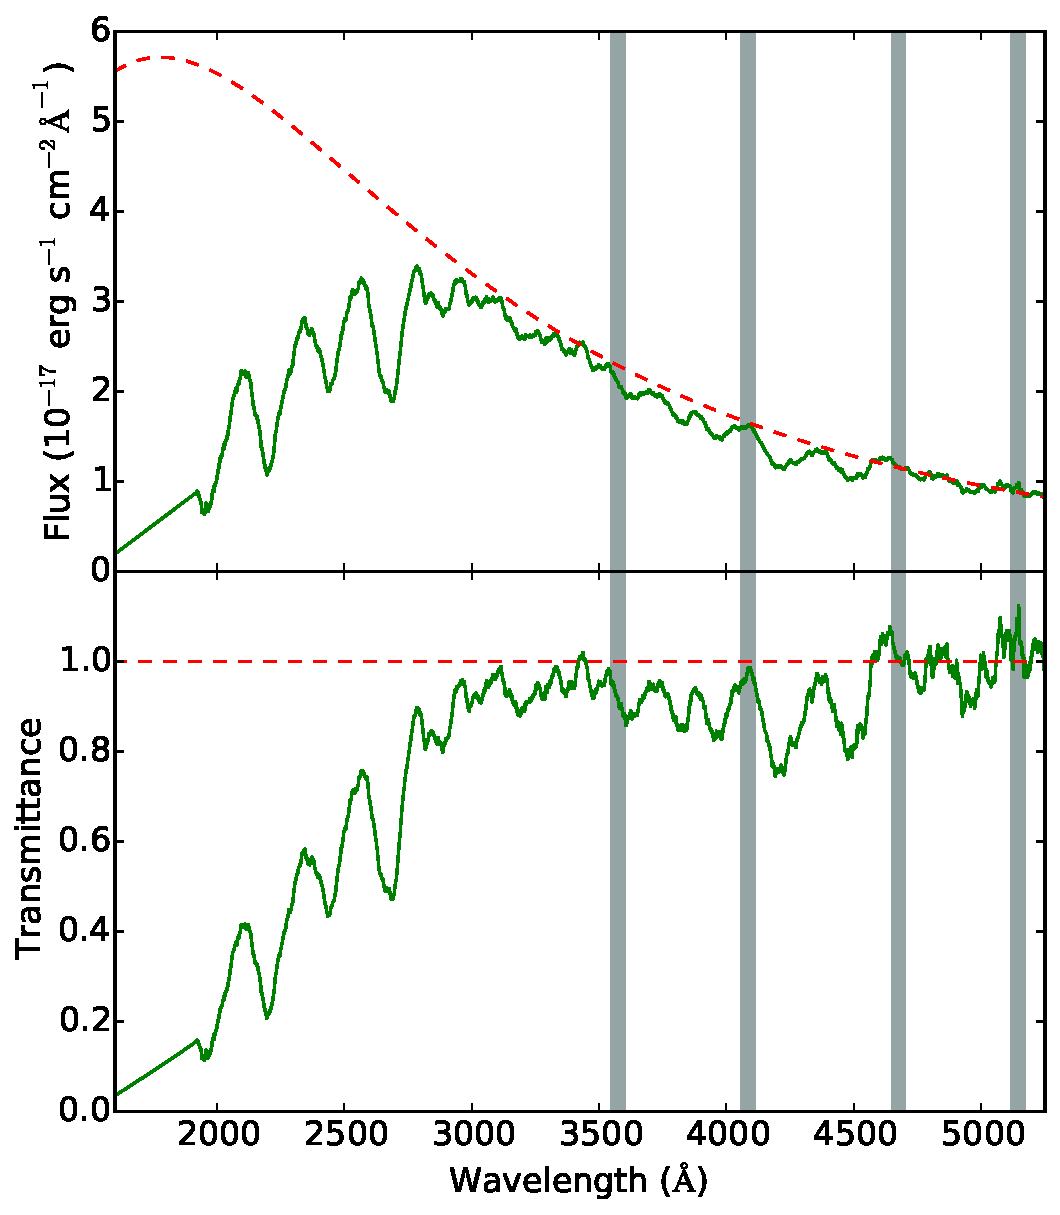
\includegraphics[scale=0.4]{figures/specTemplate}
\caption{iPTF13ajg is fitted with the Planck function. The spectrum of iPTF13ajg (green) can shows a good agreement with the black body (red) at $\lambda>3000\AA$. At lower wavelengths a strong deviation from the model is observed, highlighting the need for a correction to the model. The ratio between the observed spectrum and the continuum give a measure of the absorption strength as a function of wavelength and can be used in modelling the SLSN SED.}
\label{fig:specTemplate}
\end{figure}

\subsection{Modelling the SED evolution}
\label{sec:Magnetar}
To understand the evolution of the SED with time we must employ a model for an engine that provides the late time energy deposition needed to explain the photospheric velocity and temperature observed in SLSNe. While still a matter of active debate in literature, in recent years the birth and spin-down of a magnetar model has appeared as the strongest candidate to explain these extremely luminous events \citep{2013ApJ...770..128I,2013Natur.502..346N}. In this model, SLSNe begin as CCSN with a magnetar, a rapidly rotating, highly magnetised neutron star, born at its core. As the magnetar spins down due to the interactions with its environment, it dissipates its energy in the form of high energy radiation that is then captured by the expanding ejecta and thermalised to produce the observed blackbody SED \citep{2010ApJ...717..245K,2010ApJ...719L.204W,2012MNRAS.426L..76D}.

Following the method from \cite{2013ApJ...770..128I}, the bolometric luminosity of a SLSN as a function of time, t, can be defined using equation \ref{Eq:MagnetarLum}. This is dependant on the magnetic field of the neutron star ($B_{14}$, expressed in $10^{14}$ Gauss), its spin period ($P_{ms}$, in the unit of ms) and a diffusion time-scale parameter ($\tau_M$, expressed in days). The spin-down time scale, $\tau_P$, is defined in equation \ref{Eq:SDPeriod}. The opacity and total energy parameters have been fixed as $\kappa = 0.1cm^2g^{-1}$ and $E = 10^{51}$erg respectively. It has been shown \citep{2013ApJ...770..128I,2014ApJ...796...87I,2015MNRAS.452.3869N,2015MNRAS.449.1215P} that these parameters only weakly affect the quality of fitting and therefore can be omitted.

\begin{equation}
\label{Eq:MagnetarLum}
L(t) = 4.9\times 10^{46}\,e^{ -(t / \tau_m)^2 } \int_{0}^{t} \frac{2t'}{\tau_m^2}\,e^{(t'/\tau_m)^2}\,\frac{B_{14}^{2}\,P_{ms}^{-4}}{(1+t'/\tau_{p})^2} dt'
\end{equation}

\begin{equation}
\label{Eq:SDPeriod}
\tau_{p} = 4.7B_{14}^{-2}P_{ms}^{2}days
\end{equation}
Physically $\tau_M$ is proportional to the ejecta mass($M_{ej}$) which is sometimes chosen as the fit parameter instead. The two parameters can be converted between each other using equation \ref{Eq:Mej}, where $E$ is the explosion energy and $\kappa$ the opacity of ejecta.
\begin{equation}
\label{Eq:Mej}
M_{ej} = (\frac{\tau_{M}}{10days})^{4/3}(\frac{\kappa}{0.1cm^2g^{-1}})^{-2/3}(\frac{E_k}{10^{51}erg})^{1/3}M_{\odot}
\end{equation}
The velocity of the ejecta, $v_{core}$ is assumed to be constant and is found using the inferred mass of the ejecta, $M_{ej}$ and its kinetic energy, $E_{mag}$ (equation \ref{Eq:vcore}), which in turn depends on the explosion energy and the energy released by the spin down of the magnetar (equation \ref{Eq:Emag}). Following the work of \cite{2013ApJ...770..128I,2013Natur.502..346N,2015MNRAS.452.3869N}, constant value of $10^{51}$ erg is used as the explosion energy.
\begin{align}
\label{Eq:Emag}
E_{mag} = 4.9\times10^{46} B^2 P^{-4} \tau_{P}  \text{ erg} \\
E_k = 10^{51} + 0.5 \times E_{mag} \text{ erg}\\
\label{Eq:vcore}
v_{core} =  \sqrt{\frac{10 E_{k}}{3 M_{ej}}} \text{ cm s}^{-1}
\end{align}

In its simplest form the model only predicts the total radiated energy of the SN and does not make any predictions about the SED of the object. It is therefore most commonly used with bolometric light curves, synthesised from the photometry. \cite{2013ApJ...770..128I} shows, however, that is is possible to predict the photospheric radius of a SN based on this model.
\begin{align}
r_{core}(t) = v_{core}  t \\
\rho_{core}(t)= \frac{3 M_{ej}}{4  \pi  r_{core}^3(t)}\\
\tau_{core}(t) = \kappa  \rho_{core}(t) v_{core} t
\end{align}
While the radius of the photosphere exceeds that of the core ejecta the radius can be found using equation \ref{Eq:R19}.
\begin{equation}
\label{Eq:R19}
R(t) = r_{core}(t) \left(\frac{\alpha - 1}{\tau_{core}(t)}\right)^\frac{1}{1 - \alpha}
\end{equation}
When the photosphere recedes into the core the radius is instead found by equation \ref{Eq:R20} \citep{2013ApJ...770..128I}.
\begin{equation}
\label{Eq:R20}
R(t) = r_{core}(t) - \frac{1 - \frac{\tau_{core}(t)}{\alpha - 1}}{\kappa \rho_{core}(t)}
\end{equation}

Combining this with the total luminosity and the assumption that the object radiates as a blackbody gives us the photospheric temperature. Feed this into the Planck equation gives an approximation for the SED of a SLSN. This method allows for the magnetar model to be fit directly to the multi-band photometry without the need to produce the pseudo-bolometric light curves. We combine this with the absorption templates to produce a model of the SLSN spectral evolution as a function of time.

\subsection{Magnetar model}
Early studies used a simple expanding photosphere radiating as a
cooling black body to represent the SLSN-I light curves \citep[eg.
][]{2013ApJ...779...98H}. This approach provides a good approximation
around the peak of the light curve, but it begins to significantly
deviate from the data at 30 days after maximum light
(Fig.~\ref{fig:PS1-11ap}).  Instead we use the currently popular
magnetar model, which is able to reproduce the photometric behaviour
for the entire SLSN-I population
\citep{2013ApJ...770..128I,2013Natur.502..346N}, in particular at late
times.

In the magnetar model, the bolometric luminosity, $L$, as a function
of time $t$ for a homologously expanding ejecta is
\citep{1982ApJ...253..785A}
\begin{equation}
L(t) = 4.9\times 10^{46}\,e^{ -(t / \tau_\mathrm{m})^2 }\delta(t) \int_{0}^{t} \frac{2t'}{\tau_\mathrm{m}^2}\,e^{(t'/\tau_\mathrm{m})^2}\,\frac{B_{14}^{2}\,P_{\mathrm{ms}}^{-4}}{\left(1+t'/\tau_\mathrm{p}\right)^2} dt',
\label{Eq:MagnetarLum}
\end{equation}
where $\tau_\mathrm{m}$ is the diffusion timescale, $B_{14}$ is the
neutron star magnetic field in units of $10^{14}$\,G,
$P_{\mathrm{ms}}$ is the magnetar spin period in ms, $\delta(t)$ is
the deposition function or trapping coefficient, and $\tau_\mathrm{p}$
is the magnetar spin-down timescale, inferred from $B_{14}$ and
$P_{\mathrm{ms}}$ \cite[see Appendix D of ][and references therein for
full details]{2013ApJ...770..128I}.

The trapping coefficient, $\delta(t)$, is often assumed to be unity
(i.e., implying the full trapping of the high-energy photons radiated
by the magnetar within the supernova ejecta) and time-independent
\citep{2013ApJ...770..128I,2015MNRAS.449.1215P,2015MNRAS.452.3869N}.
Here we use a correction introduced by \cite{2015ApJ...799..107W} with
a time-dependent trapping coefficient of
\begin{equation}
\delta(t) = 1 - \exp\left({-\frac{9\kappa \mathrm{M}_{\mathrm{ej}}^{2}}{40\pi  E_k} t^{-2}} \right),
\label{Eq:Wang}
\end{equation}
where $\mathrm{M}_{\mathrm{ej}}$ is the ejecta mass, $E_k$ is the
explosion energy, and $\kappa$ is the opacity.
$\mathrm{M}_{\mathrm{ej}}$ is proportional to $\tau_\mathrm{m}$, $E_k$
and $\kappa$ \citep{2013ApJ...770..128I}. We fix the explosion energy
to be $E_k = 10^{51}$\,erg and the opacity as $\kappa =
0.1$\,cm$^2$g$^{-1}$ following other studies
\citep[e.g.][]{2013ApJ...770..128I,2014ApJ...796...87I,2015MNRAS.452.3869N,2015MNRAS.449.1215P}.
Using this time-dependent trapping coefficient improves the late-time
fit to the light curve.  For a typical SLSN we calculate $\delta
\simeq 1$ up to 75 days post explosion. However, as the ejecta opacity
to high energy photons decreases with time we find $\delta \simeq 0.8$
at 150 days post explosion, emphasising the importance of this
correction in the late time light curves.

We use the equations derived in Appendix D of
\cite{2013ApJ...770..128I} to relate the magnetar model parameters
described above to the photospheric radius and temperature and their
time evolution. The photospheric radius is proportional to the ejecta
velocity, which is also a function of the kinetic energy and
$\mathrm{M}_{\mathrm{ej}}$. Thus, using Planck's law the magnetar
model parameters can also be used to generate a simple smooth SED. In
the next section, we discuss how we adjust this SED to physically
resemble the spectra of SLSNe-I.


\begin{figure}
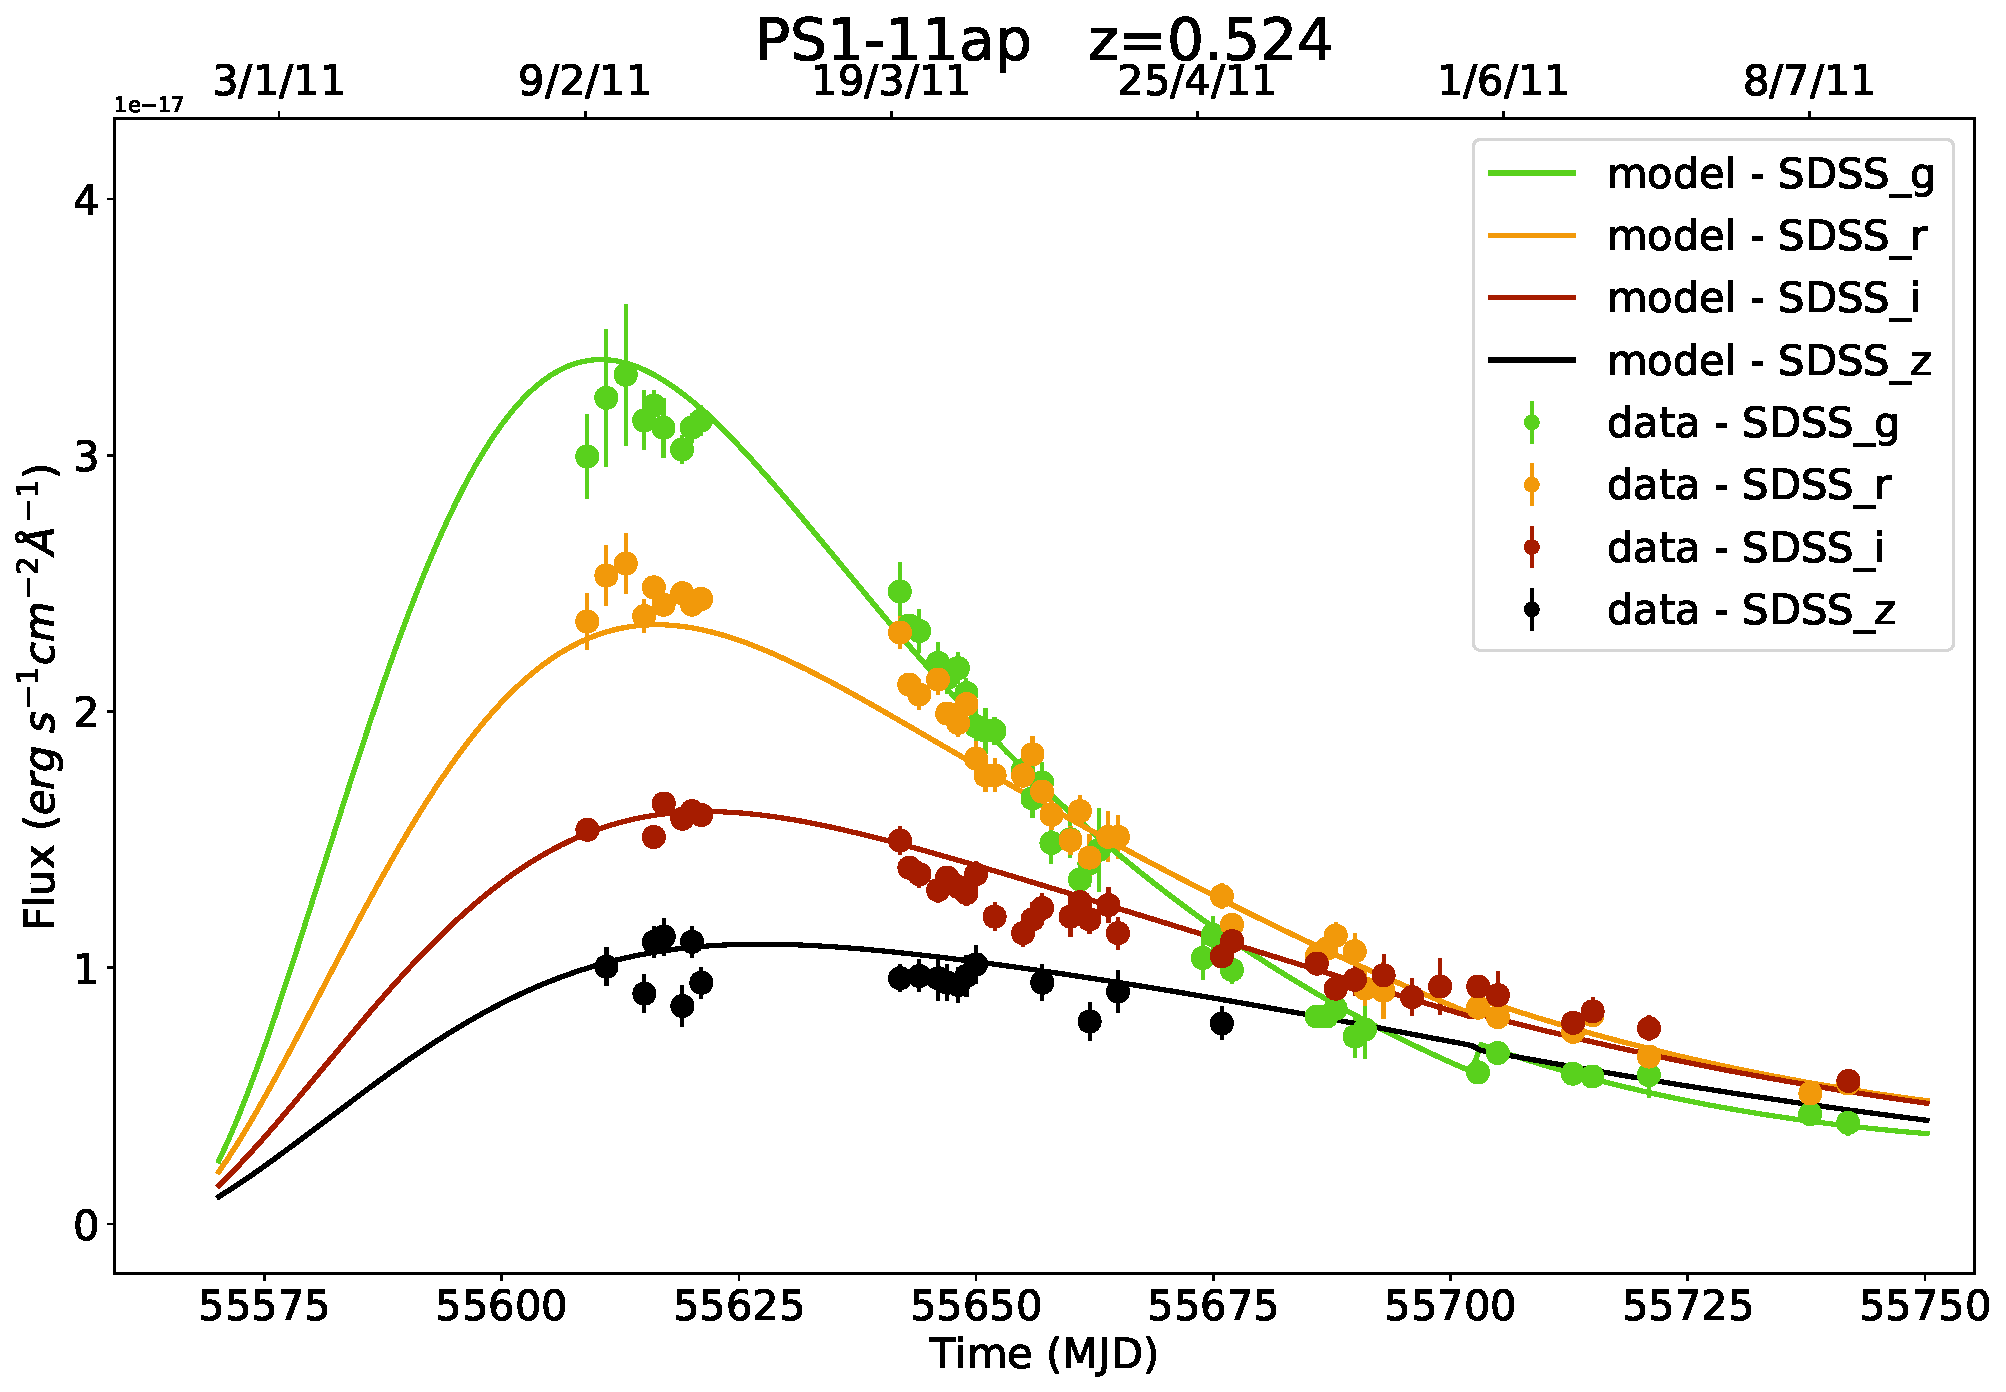
\includegraphics[scale=0.5]{figures/PS1-11ap}
\caption{The SLSN-I PS1-11ap $griz$ light curve
  \citep{2014MNRAS.437..656M} compared to two models describing its
  photometric evolution. In the upper panel, the model is a simple
  expanding and cooling black body fitted to data around maximum light
  only, and in the lower panel the model is our `absorbed' magnetar
  model fitted to the entire light curve. In the case of the magnetar model, the spectrum of
  SNLS-06D4eu \citep{2013ApJ...779...98H} has been used as an
  absorption template in the modelling of the SED (see Section
  \ref{sec:KCorrection}). Note that while both models can produce
  reasonable fits around the peak of the light cuve, the black body
  model is not able to reproduce the characteristic late-time
  behaviour of SLSNe. Light curve phases are measured with respect to peak brightness in the rest-frame \textit{u}-band as predicted by our magnetar model fit.}
\label{fig:PS1-11ap}
\end{figure}

\subsection{SED templates}
\label{sec:KCorrection}

The spectra of SLSNe-I are relatively featureless in the rest-frame
optical, with characteristic broad lines of \ion{O}{ii}, and evolve slowly
\citep{2011ApJ...743..114C,2013ApJ...779...98H,2015MNRAS.449.1215P,2014ApJ...797...24V}.
However, there are much stronger absorption features in the rest-frame
ultraviolet (UV), with features attributed to \ion{Mg}{ii},
\ion{Fe}{iii}, \ion{C}{ii}, \ion{Co}{iii}, \ion{Si }{iii} and
\ion{Ti}{iii} \citep[see][for line
identifications]{2016MNRAS.458.3455M}. This UV SED is of prime
importance for our study, as it is redshifted into the optical at high
redshift where our search is most sensitive and where we probe the
largest volume. Thus it is important to construct our magnetar model
with an appropriate SED for our $k$-corrections to be realistic.


The number of SLSNe-I with good UV coverage remains small. We
construct SED templates from three example SLSN which have a good
coverage in the UV: iPTF13ajg \citep{2014ApJ...797...24V}, SCP06F6
\citep{2009ApJ...690.1358B} and SNLS-06D4eu
\citep{2013ApJ...779...98H}. In each case we use one spectrum per
object, as spectral time series are only available for iPTF13ajg and
SCP06F6; for these objects we use the spectrum closest to maximum
light. Our spectral templates cover a rest-frame wavelength range of
1620--3320\,\AA\ (SNLS-06D4eu), 1800--3800\,\AA\ (SCP06F6) and
1800--5250\,\AA\ (iPTF13ajg).

We follow \cite{2014ApJ...797...24V}, fitting Planck's law to several
featureless, 50\,\AA\ wide, continuum regions in the observed spectra
of our three events with a good UV coverage
(Fig.~\ref{fig:specTemplate}), in order to estimate the black body
continuum. We then use the ratio between the observed spectra and
these blackbody continua as measure of the strength of the absorption
features as a function of wavelength in the different spectra. The
result is a multiplicative function that, when combined with a black
body continuum from Planck's law, can reproduce an observed SLSN-I
spectrum on any epoch (Fig.~\ref{fig:specTemplate}). We assume
that the red part of the optical SED not covered by our templates
follows a black body, and for the blue part we linearly extrapolate the
SEDs to lower wavelengths from the bluest 200\AA~of the template (Fig.~\ref{fig:specTemplate}).
This combination of the magnetar model and our UV SED templates
results in a significant improvement in the light curve fits
compared to the simpler expanding and cooling black body model
(Fig.~\ref{fig:PS1-11ap}).


\begin{figure}
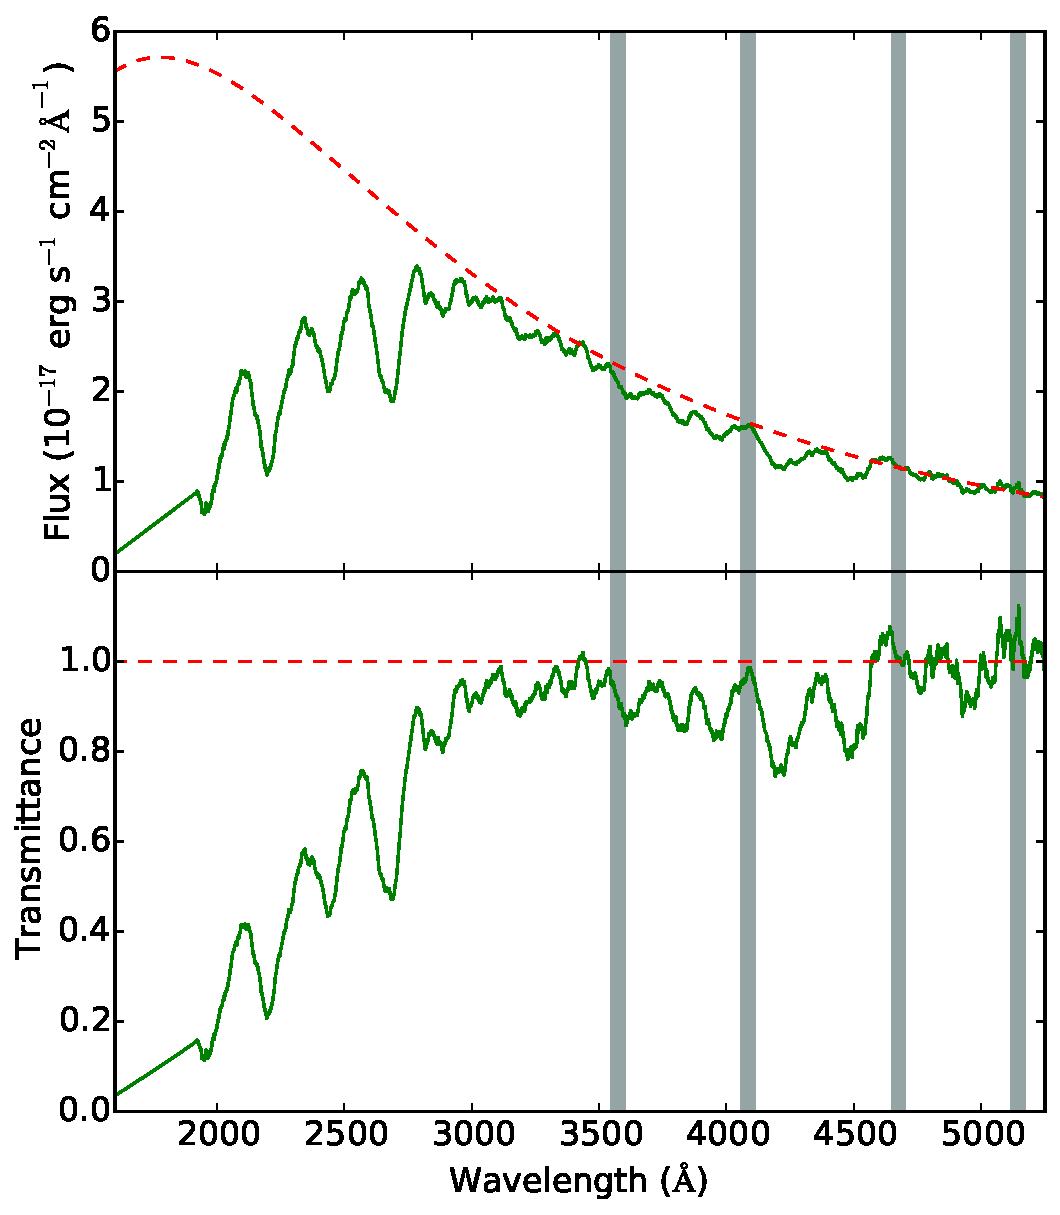
\includegraphics[scale=0.5]{figures/specTemplate}
\caption{Contructing template SEDs for SLSNe-I. Upper panel: the
  spectrum of iPTF13ajg \citep[solid;][]{2014ApJ...797...24V} fitted to
  Planck's law (dashed) in narrow, 50\,\AA, continuum regions (vertical
  bands).  There is a good agreement between the black body and
  the data in the region $\lambda>3000$\,\AA, with stronger absorption
  features appearing further blueward. Lower panel: the ratio between
  the observed spectrum and the continuum fit giving the absorption
  strength as a function of wavelength. This can then be used to
  improve the accuracy of the UV SED by combining it with a time
  dependent black body (Section \ref{sec:KCorrection}).}
\label{fig:specTemplate}
\end{figure}

\subsection{SLAP}
text
\subsection{Optimisation}
text
\subsubsection{Least-Squares fitting}
text
\subsubsection{\textsc{MultiNest}}
text
\subsection{pyMagnetar}
text

\section{Searching for Fast Transients}
text
\subsection{Searching for Bumps of SLSNe}
text
\subsection{Searching for Rapidly Evolving Transients}
text

\section{Modeling CCSN}
text
\subsection{CoCo}
text
\subsection{pyCoCo}
text
\subsection{SNIb/c SED UV Extensions}
text
\subsection{SNII with CoCo}
text

\section{Gaussian Processing}
text
\subsection{Theory}
text
\subsection{Choice of Kernels}
text
\subsection{Interpolating Light Curves}
text
